\chapter{فعالیت‌ها و تجربیات کارآموزی}

در این قسمت به تجربیات کسب شده در دوره کارآموزی شرکت عصر‌گویش‌پرداز پرداخته خواهد شد. در این دوره کارآموزی، در پروژه بازشناسی گفتار به واسطه صوت و تصویر (پرشین ای-وی-اس-آر
\LTRfootnote{PersianAVSR}
) فعالیت داشته‌ام. در ادامه، فعالیت‌های انجام شده در این پروژه به تفصیل بیان خواهد شد.

\section{پروژه پرشین ای-وی-اس-آر}

در این بخش، در ابتدا به صورت خلاصه مساله و ضرورت حل آن بررسی خواهد شد سپس به بررسی فعالیت‌های انجام شده در جهت حل این مساله و آماده‌سازی یک خدمت
\LTRfootnote{Service}
برای ارائه آن، پرداخته خواهد شد.

\subsection{مساله بازشناسی گفتار}

مهم‌ترین راه ارتباطی انسان، زبان و یکی از ارکان مهم آن، گفتار می‌باشد. بنابراین یکی از مناسب ترین روش‌ها برای ارتباط و تعامل با رایانه‌ها، گفتار می‌باشد. به همین دلیل این مساله، یکی از مهم‌ترین مسائل عصر حاضر می‌باشد. 

رویکرد غالب در جهت حل این مساله، ایجاد سامانه‌ای است که با دریافت گفتار به صورت سیگنال‌های صوتی، آن را درک کند و سپس متن متناظر با گفتار را به عنوان خروجی، برگرداند. این رویکرد، عملکرد مناسبی در موقعیت‌های بدون نویز از خود نشان می‌دهد اما در صورت قرارگیری در محیط‌ها و موقعیت‌های نویزی، دچار افت کیفیت شده و عملکرد ضعیفی از خود نشان می‌دهند.

برای حل این مساله دو رویکرد عمده وجود دارد:
\begin{itemize}
	\item تقویت گفتار
	\LTRfootnote{Speech Enhancement (SE)}
	\item بازشناسی گفتار با استفاده از ترکیب داده‌های صوتی و بصری
	\LTRfootnote{Audio-Visual Speech Recognition (AVSR)}
\end{itemize}

در این پروژه، برای افزایش پایداری
\LTRfootnote{Robustness}
مدل های بازشناسی گفتار در محیط‌های نویزی، از رویکرد دوم استفاده شده است. در این رویکرد، مدل تلاش می‌کند با استفاده از داده‌های بصری - به خصوص حرکت لب‌های فرد گوینده - ضعف قسمت‌های نویزی سیگنال‌های صوتی را جبران کرده و عملکرد بهتری از خود نشان دهد.

\subsection{بررسی پیشینه}

اولین گام در این دوره کارآموزی، مرور سوابق پژوهشی در جهت حل این مساله بوده است. برای یافتن مقالات مربوط به این مساله، با استفاده از سایت پیپرزویدکد
\LTRfootnote{Papers With Code (https://paperswithcode.com)}
، گوگل اسکولار
\LTRfootnote{Google Scholar (https://scholar.google.com)}
و کانکتدپیپرز
\LTRfootnote{Connected Papers (https://connectedpapers.com)}
فرایند جستجو مقالات را آغاز کرده و در نهایت مقالات مرتبط را با در نظر گرفتن پارامتر‌های زمان انتشار، وجود پیاده‌سازی در سایت گیت‌هاب
\LTRfootnote{Github (https://github.com)}
 و وجود مدل‌های آماده، جمع‌آوری و در یک برگه گوگل ذخیره کردم. لیست مقالات جمع‌آوری شده، در پیوست قابل مشاهده می‌باشد. % در ادامه لیبل پیوست یک اضافه شود.
 
پس از جمع‌آوری تمام مقالات، برای یافتن مقاله مناسب، به بررسی تمام مقالات پرداختم. در کل، یازده مقاله جمع‌آوری شده، دارای پیاده سازی با استفاده از چارچوب‌های
\LTRfootnote{Framework}
 تنسورفلو
\LTRfootnote{Tensorflow}
و پایتورچ
\LTRfootnote{PyTorch}
بودند. از میان این یازده مقاله، به دلیل جدیدتر بودن، وجود پیاده‌سازی در گیت‌هاب و وجود مدل های آماده، مدل ای-وی هیوبرت
\LTRfootnote{Audio-Visual HuBERT (AV-HuBERT)}
 و مقاله مربوط به آن
\LTRfootnote{Robust Self-Supervised Audio-Visual Speech Recognition (https://arxiv.org/abs/2201.01763)}
را انتخاب نمودم.

\subsection{مدل خود-نظارتی ای-وی هیوبرت}

مدل ای-وی هیوبرت، یک مدل خود-نظارتی
\LTRfootnote{Self-Supervised}
می‌باشد و آموزش آن شامل دو مرحله پیش‌آموزش بر روی داده‌های بدون برچسب و کوک کردن آن با استفاده از داده‌های برچسب‌گذاری شده می‌باشد. به همین دلیل، این مدل با استفاده با حجم کم‌تری از داده‌های برچسب‌گذاری شده، عملکرد بهتری نسبت به مدل های نظارت‌شده
\LTRfootnote{Supervised}
 از خود نشان می‌دهد.

ساختار یادگیری این مدل، از رویکرد اصلی آموزش در مدل زبانی معروف برت
\LTRfootnote{Bidirectional Encoder Representations from Transformers (BERT)}
 الهام گرفته شده است. مدل زبانی برت، یک مدل مبتنی بر ترنسفورمر
 \LTRfootnote{Transformer}
  می‌باشد و برای یادگیری سعی می‌کند قسمتی از جمله ورودی - برای مثال تعدادی از کلمات موجود در جمله - را پوشانده و در ادامه با کمک کلمات مجاور و ساختار جمله، کلمات پوشانده شده را حدس بزند. این روش منجر می‌شود با حجم داده برچسب‌گذاری شده کمتر و داده‌های بدون برچسب، مدل درک مناسبی نسبت به ساختار جملات و جایگاه کلمات در جمله به دست آورد. 

با الهام از این ایده، مدل هیوبرت
\LTRfootnote{HuBERT}
برای حل مساله بازشناسی گفتار به واسطه صوت
\LTRfootnote{Automatic Speech Recognition}
پیشنهاد شده است. یکی از تفاوت های اساسی حوزه صوت و متن، ساختار داده ورودی می‌باشد. در حوزه متن، ورودی‌ها به دلیل گسسته بودن، قابل شکستن به ساختار‌های کوچک‌تر با معنی به صورت توکن
\LTRfootnote{token}
یا کلمات می‌باشند در صورتی که صوت،دارای ماهیت پیوسته بوده و به همین دلیل به طور مستقیم چنین امکانی در این حوزه وجود ندارد. برای حل این مشکل و گسسته سازی صوت و گفتار، پژوهشگران از آوا‌ها و هجاها به عنوان کوچکترین ساختار‌های معنی‌دار در این حوزه استفاده کرده و گفتار را به صورت ترکیبی از آنها تعریف کردند. 

در این مدل، برای استخراج آوا‌ها، از استخراج‌کننده ویژگی
\LTRfootnote{Feature Extractor}
ام-اف-سی-سی
\LTRfootnote{Mel-Frequency cepstrum coefficients (MFCC)}
استفاده شده است. این استخراج‌کننده ویژگی با دریافت گفتار، ویژگی‌های با ابعاد ۳۹ را در هر لحظه تولید می‌کند. در نهایت با یک الگوریتم خوشه‌بندی نظیر کا-مینز
\LTRfootnote{K-means}
آواهای اصلی مشخص شده و در فرایند آموزش به عنوان واحد‌های سازنده گفتار، شرکت می‌کنند. فرایند استخراج ویژگی، تنها در دور
\LTRfootnote{Epoch}
اول به واسطه استخراج‌کننده ویژگی ام-اف-سی-سی انجام شده و در مراحل بعدی به واسطه بازنمایی موجود در لایه‌های میانی شبکه کد‌کننده
\LTRfootnote{Encoder}
ترنسفورمر انجام می‌شود.

در ادامه برای یادگیری مدل، بخشی از آواها و هجاهای اصلی که در فرایند خوشه‌بندی مشخص شده‌اند، در گفتار ورودی پوشانده شده و مدل تلاش می‌کند تا با توجه به ارتباط میان آواها و یادگیری ساختار آنها، بخش پوشانده را حدس بزند. در این روش، از تابع خطا آنتروپی متقاطع
\LTRfootnote{Cross Entropy}
و الگوریتم‌های بهینه‌سازی نظیر الگوریتم آدام
\LTRfootnote{Adam}
استفاده شده است.

\begin{figure}[!h]
	\centering
	\captionsetup{justification=centering}
	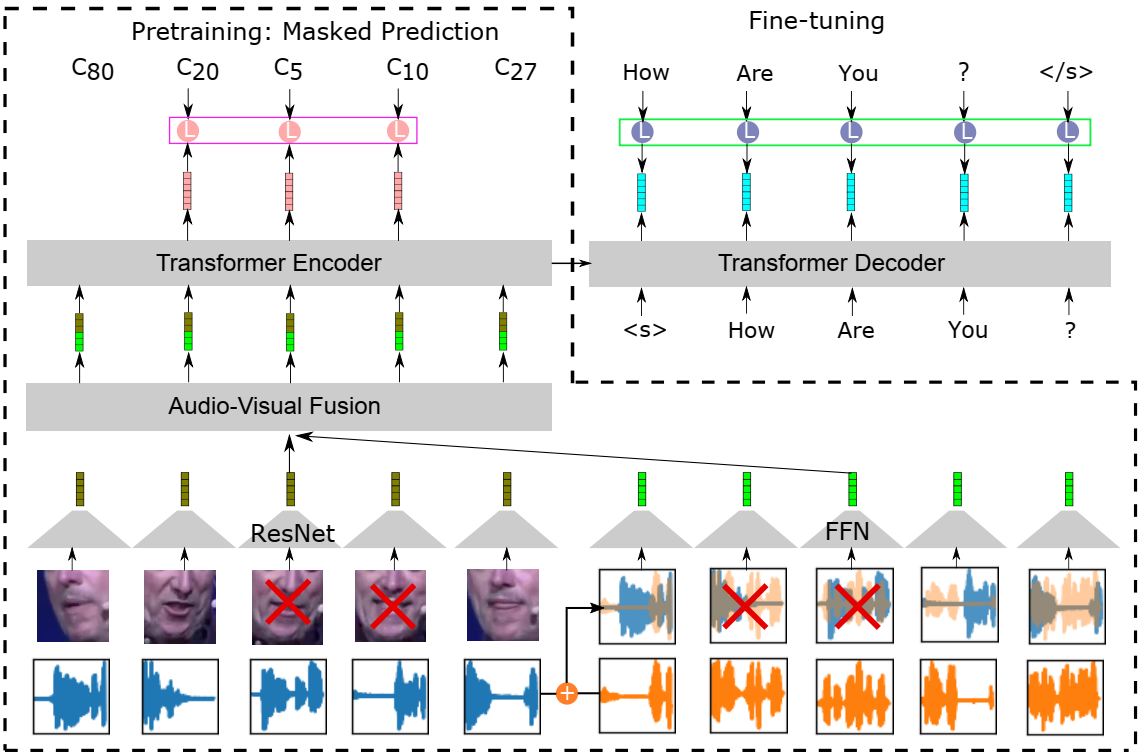
\includegraphics[width=\textwidth]{images/av-hubert-model}
	\caption[معماری مدل ای-وی هیوبرت]{معماری مدل ای-وی هیوبرت \cite{shi2022robust}}
	\label{fig:av-hubert-model}
\end{figure}

مدل ای-وی هیوبرت، بر پایه مدل هیوبرت ارائه شده است و رویکردی مشابه را این‌بار برای حل مساله بازشناسی گفتار به واسطه صوت و تصویر در پی می‌گیرد. همانطور که در تصویر 
\ref{fig:av-hubert-model}
مشاهده می‌شود، در این مدل فریم‌های صوتی و بصری ویدیو، به ترتیب به واسطه کدکننده صوتی و کدکننده بصری به یک بازنمایی متراکم
\LTRfootnote{Dense Representation}
تبدیل می‌شوند.

در کدکننده بصری، از یک مدل رزنت-هجده 
\LTRfootnote{ResNet-18}
شده است. مدل های رزنت، به جای ساختار ترتیبی لایه‌ها، دارای اتصالات خارج از ترتیب بوده که موجب کاهش مشکل محوشدن گرادیان
\LTRfootnote{Vanishing Gradient}
و به تبع آن، افزایش تعداد لایه‌های مدل می‌شود. این نوع از مدل‌ها، پیش از ارائه مدل‌های مبتنی بر ویژن‌ترنسفورمر
\LTRfootnote{Vision Transformer (ViT)}
، دارای بهترین عملکرد در حوزه تصویر بوده‌اند. پیش از ورودی دادن فریم‌های بصری ویدیو به این مدل رزنت-هجده، تغییرات زیر بر روی تصویر اعمال می شود.

\begin{itemize}
	\item ۶۸ نقطه کلیدی چهره تشخیص داده شده و سپس به واسطه یک تبدیل خطی، این نقاط کلیدی به یک دستگاه مختصات متمرکز بر چهره انتقال پیدا می‌کند.
	\item یک منطقه مورد علاقه
	\LTRfootnote{Region of Interest (ROI)}
	با ابعاد ۹۶×۹۶ حول دهان فرد در چهره بریده می‌شود.
	\item کانال‌های رنگی تصویر به سطح خاکستری منتقل می‌شوند.
	\item در جهت داده‌افزایی
	\LTRfootnote{Data Augmentation}
	یک کادر با ابعاد ۸۸×۸۸ به صورت تصادفی از منطقه مورد علاقه بریده شده و به صورت تصادفی به صورت افقی قرینه
	\LTRfootnote{Horizontal Flip}
	می شود.
\end{itemize}

به دلیل تاثیر بیشتر داده‌های صوتی نسبت به داده‌های بصری در این مساله، برای کاهش تاثیر داده‌های صوتی و افزایش تاثیر داده‌های بصری در یادگیری مدل، از یک شبکه تماما متصل عصبی استفاده شده است. فریم‌های صوتی خام ورودی، پیش از ورودی داده شدن به شبکه عصبی، به واسطه یک استخراج کننده ویژگی خاص
\LTRfootnote{Log Filterbank Energy}
به یک بردار ۲۶ بعدی با فاصله ۱۰ میلی‌ثانیه تبدیل می‌شود. علاوه بر این، به دلیل تفاوت نرخ برداشت فریم های صوتی و بصری - فریم‌های صوتی با فرکانس صد هرتز و فریم‌های بصری با فرکانس ۲۵ هرتز برداشت می‌شود - به ازای هر فریم بصری،چهار فریم صوتی برداشت می‌شود تا هماهنگی زمانی میان دو نوع داده حفظ شود.

پس از ایجاد یک بازنمایی متراکم از فریم‌های صوتی و بصری ویدیو، این بازنمایی به عنوان ورودی به لایه‌های کدکننده ترنسفورمر داده می‌شود. همانطور که در مدل زبانی برت و مدل بازشناسی گفتار هیوبرت توضیح داده شد، در اینجا نیز شبکه کدکننده به دنبال حدس آواهای پوشانده شده است و تلاش می‌کند با این کار، ماهیت و ارتباط میان آواها را به صورت بدون نظارت درک کند. در این مرحله، با استفاده از داده‌های بدون برچسب، می‌توان پیش‌آموزش
\LTRfootnote{Pre-Train}
مدل را انجام داد و در نهایت برای تکمیل فرایند یادگیری مدل و انتقال دانش کسب شده در فرایند پیش‌آموزش به مساله اصلی، مدل با استفاده از داده‌های برچسب‌خورده، کوک می‌شود. برای این انتقال دانش، از یک شبکه کدبرگردان
\LTRfootnote{Decoder}
ترنسفورمری به همراه تابع زیان سی-تی-سی
\LTRfootnote{Connectionist Temporal Classification Loss (CTC Loss)}
 استفاده می‌شود.
 
 \subsection{دادگان‌های صوتی-تصویری موجود}
 
 پیش از ارائه مدل‌های خود-نظارتی یا نیمه-نظارت‌شده، رویکرد غالب مدل‌ها در جهت حل مساله بازشناسی گفتار به واسطه صوت و تصویر، مبتنی بر مدل‌های نظارت‌شده بوده است. به همین دلیل، عملکرد و دقت این مدل‌ها به حجم دادگان وابسته بوده و در صورت محدود بودن آن، کیفیت و عملکرد پایینی از خود نشان می‌دادند.
 
 با توجه به این توضیحات، بررسی دادگان‌های موجود ضروری به نظر می‌رسد. در ادامه، به صورت مختصر شرحی در رابطه با مشخصات دادگان‌های ال-آر-اس دو و سه
 \LTRfootnote{LRS2-BBC, LRS3-TED}
و وکس-سلب
 \LTRfootnote{Vox-Celeb}
بیان خواهد شد.
   
\subsubsection{دادگان ال-آر-اس دو و سه}

دادگان ال-آر-اس دو، یکی از بزرگ‌ترین دادگان‌های موجود برای مساله لب‌خوانی می‌باشد. این دادگان با استفاده از برنامه‌های تلویزیونی - به ویژه اخبار و برنامه‌های گفتگومحور
\LTRfootnote{Talk Show}
- شبکه انگلیسی زبان بی-بی-سی
\LTRfootnote{BBC}
تشکیل شده است. پس از ارائه این دادگان، دادگان دیگری با نام ال-آر-اس سه، این‌بار با استفاده از ویدیو‌های سخنرانی‌های برنامه‌های تد
\LTRfootnote{TED}
و تد-ایکس
\LTRfootnote{TEDx}
توسط محققان دانشگاه آکسفورد
\LTRfootnote{Oxford University}
منتشر شد. این دو دادگان، از بزرگ‌ترین دادگان‌های برچسب‌گذاری شده به زبان انگلیسی می‌باشند و معیار ارزیابی
\LTRfootnote{Benchmark}
در مساله بازشناسی گفتار به واسطه صوت و تصویر محسوب می‌شوند.

\subsubsection{دادگان وکس-سلب}

 این دادگان، یک دادگان چند‌زبانه است که در ابتدا برای مساله تشخیص گوینده چندزبانه با استفاده از داده‌های صوتی و بصری ارائه شده است. بر روی هم، این دادگان شامل بیش از دو هزار و ۴۴۲ ساعت گفتار از بیش از شش هزار گوینده که از سایت اشتراک‌گذاری ویدیو یوتیوب
\LTRfootnote{YouTube}
استخراج شده است، می‌باشد. همچنین، این دادگان شامل زیرنویس و متن اصلی که در ویدیو‌ها بیان می‌شود، نمی‌باشد. مزیت این دادگان نسبت به دادگان ال-آر-اس دو و سه، تنوع بیشتر موقعیت‌ها و صحنه‌هایی است که وجود دارد. 
 
\subsection{ایجاد دادگان فارسی}

با توجه به توضیحات داده شده در بخش قبل، دادگان‌های موجود برای حل مساله بازشناسی گفتار به واسطه صوت و تصویر، غالبا به زبان انگلیسی بوده و در زبان فارسی قابل استفاده نمی‌باشند. به همین دلیل، در این دوره تصمیم به ایجاد و جمع‌آوری یک دادگان فارسی گرفتیم.

پیش از شروع فرایند جمع‌آوری ویدیو‌ها، مقالات متناظر با دادگان‌های ال-آر-اس سه و وکس-سلب را مطالعه کردم. با توجه به نکات ذکر شده در این مقالات، می‌بایست به سوالات زیر جواب داده می‌شد:

\begin{itemize}
	\item منبع جمع‌آوری ویدیو‌ها
	\item چگونگی استخراج ویدیو‌ها
	\item چگونگی پردازش ویدیو‌ها
	\item چگونگی فرایند برچسب‌زنی داده‌های استخراج‌شده
\end{itemize}

\subsubsection{منبع جمع‌آوری ویدیو‌ها}

با توجه به این موضوع که داده‌های دادگان‌های مطرح انگلیسی، با استفاده از برنامه‌های تلویزیونی و ویدیو‌های اشتراک گذاشته شده در سایت اشتراک‌گذاری ویدیو یوتیوب به دست آمده بودند، گزینه‌های زیر از گزینه‌های مطرح برای جمع‌آوری ویدیو‌های فارسی بودند:

\begin{itemize}
	\item سایت تلوبیون
	\item سایت آپارات
	\item سایت یوتیوب
	\item شبکه اجتماعی توییتر
	\LTRfootnote{Twitter}
	\item شبکه اجتماعی اینستاگرام
	\LTRfootnote{Instagram}
	\item سایت‌های آموزش ویدیویی نظیر فرادرس و مکتب‌خونه
\end{itemize}

در نهایت، از میان این گزینه‌ها، سایت تلوبیون به دلیل برخورداری از ویدیو‌های برنامه‌های تلویزیونی و نیازمندی به پالایش کمتر داده‌های این سایت، انتخاب شد. بنا به الگوگیری از دادگان ال-آر-اس دو و سه، در این مرحله تصمیم نهایی بر استخراج ویدیو‌های آرشیوی شبکه خبر صدا و سیما جمهوری اسلامی ایران شد.

در ادامه برای ارتقای این دادگان، می‌توان از داده‌های ویدیویی دیگر برنامه‌های تلویزیون به خصوص برنامه‌های گفتگومحور دیگر شبکه‌های صدا و سیما جمهوری اسلامی ایران نیز استفاده نمود، اما در این مرحله به دلیل محدود بودن زمان این عمل به نسخه‌های بعدی این دادگان موکول شده است.

\subsubsection{چگونگی استخراج ویدیو‌ها}

برای استخراج ویدیو‌های آرشیو تلویزیون از سایت تلوبیون، یک اسکریپت به زبان پایتون
\LTRfootnote{Python}
و با استفاده از کتابخانه سلنیوم
\LTRfootnote{Selenium}
توسعه داده شده است. زبان پایتون یکی از زبان‌های مفسری
\LTRfootnote{Interpreter}
مطرح می‌باشد. علاوه بر این، کتابخانه سلنیوم، اجازه استفاده به صورت خودکار از مرورگر را به توسعه‌دهندگان داده و توانایی خودکار سازی فرایند‌های مرورگر را با استفاده از زبان‌های برنامه‌نویسی دیگر می‌دهد.

از دیگر گزینه‌های مطرح برای انجام فرایند استخراج ویدیو‌ها، استفاده از کتابخانه ریکوئستز
\LTRfootnote{requests}
و بیوتیفول سوپ
\LTRfootnote{BeautifulSoup}
بوده است. با این حال، به دلیل بارگذاری کند
\LTRfootnote{Lazy Loading}
سایت تلوبیون، امکان استفاده از این کتابخانه‌ها وجود نداشت و به همین دلیل از کتابخانه سلنیوم برا انجام این کار استفاده شده است.

این اسکریپت با استفاده از یک برنامه راه‌اندازی
\LTRfootnote{Driver}
مربوط به مرورگر، با مرورگر متصل شده و سپس فرایند اتوماسیون و خودکار سازی را شروع می‌کند. این اسکرپیت در ابتدا، با توجه به ورودی تعیین شده به تعداد روز‌های تعیین شده، از آرشیو ویدیو‌های امروز شروع کرده و به تدریج به سراغ ویدیو‌های روز‌های قبل رفته و لینک‌های دانلود مربوط به هر ویدیو را استخراج کرده و در یک فایل متنی، ذخیره می‌کند. علاوه بر این، پس از استخراج لینک‌های دانلود ویدیو‌ها، توانایی شروع دانلود ویدیو‌ها را در اختیار دارد.

\subsubsection{چگونگی پردازش ویدیو‌ها}

ویدیو‌ها پس از دانلود، می‌بایست پردازش شده تا آماده ورودی داده شدن به مدل شوند. در این قسمت با بررسی اسکریپت‌های موجود به صورت عمومی، متوجه شدیم که خط لوله
\LTRfootnote{Pipeline}
پردازشی مربوط به دادگان وکس-سلب به صورت عمومی در سایت گیت‌هاب منتشر شده است و بدون تغییر قابل استفاده می‌باشد. این خط لوله، مربوط به مدل صوتی-تصویری سینک‌نت
\LTRfootnote{SyncNet}
می‌باشد که برای هماهنگ کردن حرکت لب‌های فرد گوینده و صوت استفاده می‌شود.

در این مدل، با استفاده از چارچوب پایتورچ و مدل‌های تشخیص چهره آماده با نام اس-سه-اف-دی
\LTRfootnote{S3FD}
چهره‌های موجود در تصویر تشخیص داده شده و در طول ویدیو دنبال می‌شوند. و در نهایت، تمامی چهره‌های موجود در ویدیو، به صورت ویدیو‌هایی از ویدیو اصلی جدا شده و برای استفاده در حل مسائل دیگر نظیر مساله بازشناسی گفتار به واسطه صوت و تصویر قابل استفاده می‌باشد. در تصویر 
\ref{fig:syncnet-sample}
چهار نمونه از خروجی‌های خط لوله پردازشی مدل سینک‌نت را مشاهده می‌کنید.

\begin{figure}[!h]
	\centering
	\captionsetup{justification=centering}
	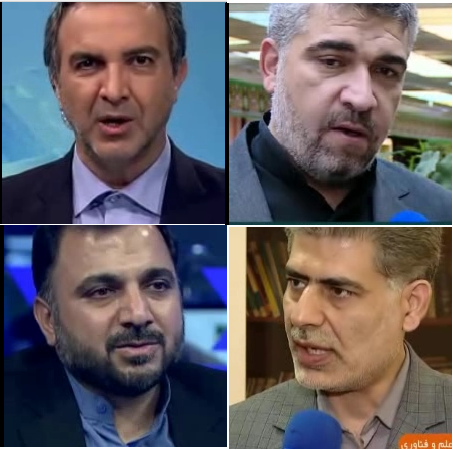
\includegraphics[width=9cm]{images/syncnet-sample}
	\caption{چهار نمونه از خروجی‌های خط لوله پردازشی مدل سینک‌نت}
	\label{fig:syncnet-sample}
\end{figure}

پیش از استفاده از این خط لوله پردازشی، به دنبال توسعه یک خط لوله از ابتدا بوده‌ام. برای این کار، ابتدا از مدل ام-تی-سی-ان-ان
\LTRfootnote{MTCNN}
که یک مدل تشخیص چهره با قابلیت آشکارسازی در یک صحنه
\LTRfootnote{Single Shot Detector (SSD)}
می‌باشد، استفاده کردم. این مدل قابلیت تشخیص چندین چهره در یک تصویر را داشته است. علاوه بر تشخیص کادر چهره فرد، قادر به تشخیص نقاط کلیدی چهره از جمله محل چشمان، محل لب و محل بینی فرد نیز بوده است.

با این حال، به دلیل دقت بالاتر و سادگی پیاده‌سازی خط لوله مربوط به مدل سینک‌نت، استفاده از این مدل آماده را برای پردازش نهایی ویدیو‌ها برگزیدم.

البته در فرایند پردازش ویدیو‌ها، دسته‌ای از خروجی‌های این مدل به اشتباه استخراج شده و نیازمند حذف در مرحله بعدی می‌باشند. حالت کلی این ویدیو‌های به اشتباه استخراج شده به شکل زیر می‌باشد:

\begin{itemize}
	\item ویدیو‌هایی که فرد صحبت نمی‌کند ولی به دلیل وجود گفتار پس‌زمینه به اشتباه استخراج شده است.
	\item ویدیو‌هایی که فرد گوینده، ماسک به صورت داشته است.
	\item ویدیو‌هایی که دارای صدای دوبله‌شده می‌باشد. برای نمونه ترجمه مترجم بر روی صحبت‌های یک فرد غیر فارسی زبان.
\end{itemize}

از آنجایی که این نوع از ویدیو‌های خروجی، از احتمال رخداد پایینی برخوردارند، می‌توان یکی از دو رویکرد زیر را در مواجهه با آنها در پیش گرفت:

\begin{itemize}
	\item تشخیص به صورت دستی و حذف آنها
	\item کوک کردن یک مدل به واسطه تمامی خروجی‌های مدل و تشخیص ویدیو‌های با ضریب اعتماد پایین
	\LTRfootnote{Low Confident}
\end{itemize}

با توجه به مشورت‌های انجام شده با منتور‌های این دوره، تصمیم نهایی بر این شد که رویکرد دوم اتخاذ شود. به گونه‌ای که در ابتدا تمام خروجی‌ها استخراج شده و پس از کوک کردن مدل نهایی، با یافتن ویدیو‌های با ضریب اعتماد پایین، این ویدیو‌ها بررسی شده و در صورتی که یکی از حالات ذکر شده در بالا باشند، حذف شوند.

علاوه بر این، به دلیل حجم بالای ویدیو‌های دانلود شده (حدود ۲۳۲ گیگابایت)، فرایند پردازش ویدیو به سادگی میسر نبوده است. با توجه به امکانات شرکت، سرور
\LTRfootnote{Server}
دارای کارت گرافیک
\LTRfootnote{GPU}
شرکت، دارای حافظه کافی برای انتقال کامل داده‌ها به این سرور و سپس پردازش تمامی آن‌ها وجود نداشت. به همین دلیل برای رفع این مشکل، از ارتباط میان سرور‌های شبکه به صورت محلی استفاده کرده و در هر مرحله، یک ویدیو را با استفاده از دستور اس-سی-پی
\LTRfootnote{scp}
از سرور دارای ویدیو‌ها دانلود‌شده به سرور فعلی منتقل کرده و پس از اعمال پردازش مربوطه بر روی این ویدیو، خروجی‌های میانی مربوط به این داده را در سرور پردازشی پاک کرده و خروجی نهایی را به سرور اولیه که دارای حجم ذخیره‌سازی کافی بوده است، ارسال می‌کردم. 

از آنجایی که فرایند پردازش ویدیو‌های دانلود شده فرایندی زمانبر می‌باشد و همچنین ارتباط شبکه محلی میان سرور‌های شرکت، دارای سرعت بالایی - حدود ۱ گیگابیت به ازای هر ثانیه - دارا می‌باشد، این عامل منجر به کندی تاثیر‌گذاری در سیستم نهایی نشده و قابل چشم‌پوشی می‌باشد.

\subsubsection{چگونگی فرایند برچسب‌زنی داده‌های استخراج‌شده}

داده‌های آموزشی مرتبط با مساله بازشناسی گفتار به واسطه صوت و تصویر، علاوه بر فریم‌های صوتی و بصری، نیازمند متن بیان شده در فریم‌های ویدیو نیز می‌باشند. به همین دلیل، نیاز است که پس از دانلود ویدیو‌ها و پردازش آنها، متن مرتبط با هر یک از این ویدیو‌ها استخراج شده و به عنوان برچسب این ویدیو مشخص شود. برای انجام فرایند برچسب‌زنی داده‌ها در دسترس، با توجه به مشاوره‌های انجام شده با منتور‌های دوره کارآموزی، راهکارهای زیر مطرح شده است:

\begin{itemize}
	\item جمع‌سپاری
	\LTRfootnote{Crowd Sourcing}
	داده‌های ویدیویی
	\item برچسب‌گذاری به صورت دستی توسط عوامل دوره کارآموزی
	\item استفاده از یک مدل آماده تبدیل گفتار به متن
	\LTRfootnote{Automatic Speech Recognition}
	و بررسی خروجی آن به ازای هر یک از ویدیو‌ها
\end{itemize}

با توجه به زمان محدود دوره کارآموزی، گزینه اول و دوم به دلیل زمانبر بودن، کنار گذاشته شده و تصمیم نهایی بر این شد که با استفاده از یک مدل تبدیل گفتار به متن و سپس بررسی خروجی این مدل به ازای هر ویدیو، این فرایند را سرعت بخشیده و دادگان را سریع‌تر آماده کرد.

در حال حاضر، حدود دو هزار و سیصد و نود ویدیو دانلود شده است و این تعداد ویدیو، در حال پردازش توسط خط لوله پردازشی سینک‌نت می‌باشد. به دلیل زمانبر بودن فرایند پردازشی، فعالیت فعلی در این پروژه تا به اینجا محدود شده است. پس از آماده سازی دادگان، امکان کوک کردن مدل ای-وی هیوبرت و دیگر مدل‌های آماده نیز وجود دارد و می‌توان میزان مفید بودن این دادگان فارسی جمع‌آوری شده را به طور بهتری ارزیابی کرد.

علاوه بر این، این دادگان قابل استفاده در مسائل دیگری نظیر تشخیص لب‌خوانی به زبان فارسی نیز می‌باشد و توانایی استفاده برای کوک کردن مدل‌های آماده موجود را نیز دارا می‌باشد.